%==============================================================================
%  Master Cybersecurity -- Cloud Security
%  Modernised & extended LaTeX Beamer deck, based on the existing
%  "AWS Academy Cloud Security Foundations" deck (4_Cloud Security AWS.pptx).
%
%  Author: Prof. Dr.-Ing. Sebastian Schlesinger (deck), Beamer transform 2026.
%  Level : MSc Cybersecurity.
%  Build : pdflatex -> pdflatex   (run twice for TOC / frame counts)
%          or:  latexmk -pdf cloud_security_master.tex
%
%  Design goals: clean academic look, concise slides, TikZ diagrams,
%  speaker notes as % comments, exercises + MCQs + bibliography.
%
%  Structure
%    Part I  -- Foundations (modernised from the existing AWS deck)
%      1 Cloud Security Intro
%      2 Shared Responsibility Model
%      3 IAM & Access Management        (+ E. Modern IAM integrated here)
%      4 Infrastructure Security
%      5 Data Protection
%      6 Logging & Monitoring
%      7 Incident Response
%    Part II -- Advanced Cloud Security (Master extensions)
%      A Zero Trust in Cloud Environments
%      B Container & Kubernetes Security
%      C Supply Chain Security
%      D Threat Modeling for Cloud Architectures
%      F Cloud-Native Detection & Response
%    Part III -- Exercises, MCQs, References
%==============================================================================
\documentclass[aspectratio=169,10pt]{beamer}

%----------------------------------- fonts ------------------------------------
\usepackage[T1]{fontenc}
\usepackage[utf8]{inputenc}
\usepackage{lmodern}
\usepackage{microtype}

%----------------------------------- core -------------------------------------
\usepackage{xcolor}
\usepackage{booktabs}
\usepackage{array}
\usepackage{pifont}      % \ding -- check / cross marks
\usepackage{listings}    % code / policy snippets
\usepackage{tikz}
\usetikzlibrary{arrows.meta,positioning,fit,backgrounds,shapes.geometric,%
                shapes.misc,calc,decorations.pathreplacing,chains}

%--------------------------------- palette ------------------------------------
\definecolor{awsink}{HTML}{232F3E}   % AWS "squid ink" (primary dark)
\definecolor{awsorange}{HTML}{FF9900} % AWS accent orange
\definecolor{accent}{HTML}{1B6CA8}    % academic blue
\definecolor{good}{HTML}{2E7D32}      % green
\definecolor{bad}{HTML}{C62828}       % red
\definecolor{warn}{HTML}{EF6C00}      % amber
\definecolor{paleblue}{HTML}{E8F0F7}
\definecolor{lightgray}{HTML}{ECEFF1}
\definecolor{midgray}{HTML}{546E7A}
\definecolor{codebg}{HTML}{F5F7FA}

%--------------------------------- theme --------------------------------------
\usetheme{default}
\setbeamertemplate{navigation symbols}{}
\setbeamersize{text margin left=0.7cm,text margin right=0.7cm}

\setbeamercolor{normal text}{fg=awsink}
\setbeamercolor{structure}{fg=accent}
\setbeamercolor{title}{fg=awsink}
\setbeamercolor{frametitle}{fg=awsink,bg=white}
\setbeamerfont{frametitle}{series=\bfseries,size=\large}
\setbeamerfont{title}{series=\bfseries,size=\LARGE}

\setbeamercolor{itemize item}{fg=awsorange}
\setbeamercolor{itemize subitem}{fg=accent}
\setbeamercolor{itemize subsubitem}{fg=midgray}
\setbeamertemplate{itemize item}{\small\raise0.2ex\hbox{\ding{110}}}
\setbeamertemplate{itemize subitem}{\footnotesize\raise0.2ex\hbox{\ding{228}}}
\setbeamertemplate{itemize subsubitem}{--}
\setbeamertemplate{enumerate items}[default]

% blocks
\setbeamertemplate{blocks}[rounded][shadow=false]
\setbeamercolor{block title}{fg=white,bg=accent}
\setbeamercolor{block body}{fg=awsink,bg=paleblue}
\setbeamercolor{block title alerted}{fg=white,bg=bad}
\setbeamercolor{block body alerted}{fg=awsink,bg=bad!8}
\setbeamercolor{block title example}{fg=white,bg=good}
\setbeamercolor{block body example}{fg=awsink,bg=good!8}

% frame title with accent rule underneath
\setbeamertemplate{frametitle}{%
  \vspace*{0.55em}%
  \begin{beamercolorbox}[wd=\paperwidth,leftskip=0.7cm,rightskip=0.7cm]{frametitle}%
    \usebeamerfont{frametitle}\insertframetitle%
    \ifx\insertframesubtitle\empty\else%
      \\[-0.15em]{\small\normalfont\color{midgray}\insertframesubtitle}%
    \fi%
  \end{beamercolorbox}%
  \vspace*{0.1em}\hspace*{0.7cm}{\color{awsorange}\rule{0.945\paperwidth}{1.1pt}}%
  \vspace*{-0.2em}%
}

% footline
\setbeamercolor{foot}{fg=midgray,bg=lightgray}
\setbeamertemplate{footline}{%
  \leavevmode%
  \hbox{%
    \begin{beamercolorbox}[wd=.32\paperwidth,ht=2.6ex,dp=1.1ex,leftskip=.7cm]{foot}%
      \tiny Master Cybersecurity {\color{awsorange}\textbullet} Cloud Security%
    \end{beamercolorbox}%
    \begin{beamercolorbox}[wd=.52\paperwidth,ht=2.6ex,dp=1.1ex,center]{foot}%
      \tiny\insertsectionhead%
    \end{beamercolorbox}%
    \begin{beamercolorbox}[wd=.16\paperwidth,ht=2.6ex,dp=1.1ex,rightskip=.7cm]{foot}%
      \hfill\tiny\insertframenumber\,/\,\inserttotalframenumber%
    \end{beamercolorbox}%
  }\vskip0pt%
}

% section divider slide
\AtBeginSection[]{%
  \begin{frame}[plain,noframenumbering]%
    \vfill\centering
    {\color{awsorange}\rule{0.16\paperwidth}{2.2pt}}\\[0.7em]
    {\usebeamerfont{title}\color{awsink}\insertsectionhead}\\[0.5em]
    {\color{midgray}\small Section \insertsectionnumber\ of the Cloud Security module}
    \vfill
  \end{frame}%
}

%--------------------------------- listings -----------------------------------
\lstdefinestyle{pol}{%
  basicstyle=\ttfamily\scriptsize,
  showstringspaces=false,
  breaklines=true,
  backgroundcolor=\color{codebg},
  frame=leftline,
  framerule=2.2pt,
  rulecolor=\color{awsorange},
  xleftmargin=1.1em,
  aboveskip=0.5em,belowskip=0.2em,
  stringstyle=\color{good},
  commentstyle=\color{midgray}\itshape,
  keywordstyle=\color{accent}\bfseries,
  morestring=[b]",
  morecomment=[l]{\#},
  morekeywords={Effect,Action,NotAction,Resource,Condition,Allow,Deny,%
    Principal,Version,Statement,Sid,kind,apiVersion,rules,verbs}%
}
\lstset{style=pol}

%---------------------------------- macros ------------------------------------
\newcommand{\cmark}{\textcolor{good}{\ding{51}}}
\newcommand{\xmark}{\textcolor{bad}{\ding{55}}}
\newcommand{\svc}[1]{{\color{accent}\textsf{\textbf{#1}}}}      % AWS service name
\newcommand{\term}[1]{{\color{awsink}\textbf{#1}}}
\newcommand{\link}[1]{{\color{accent}\small#1}}
% Map-to-existing-AWS-concept callout used throughout Part II
\newcommand{\bridge}[1]{%
  \begin{block}{\small\ding{43}\ Link to existing AWS concepts}\small #1\end{block}}

% TikZ reusable styles
\tikzset{
  box/.style   ={rounded corners=2pt,draw=accent,line width=0.8pt,fill=paleblue,
                 inner sep=4pt,align=center,font=\scriptsize},
  awsbox/.style={rounded corners=2pt,draw=awsink,line width=0.8pt,fill=awsink!8,
                 inner sep=4pt,align=center,font=\scriptsize},
  hot/.style   ={rounded corners=2pt,draw=bad,line width=0.9pt,fill=bad!10,
                 inner sep=4pt,align=center,font=\scriptsize},
  ok/.style    ={rounded corners=2pt,draw=good,line width=0.9pt,fill=good!10,
                 inner sep=4pt,align=center,font=\scriptsize},
  zone/.style  ={rounded corners=4pt,draw=midgray,dashed,line width=0.7pt,
                 inner sep=8pt},
  flow/.style  ={-{Stealth[length=2.2mm]},line width=0.8pt,draw=awsink},
  attack/.style={-{Stealth[length=2.2mm]},line width=0.9pt,draw=bad,dashed}
}

%---------------------------------- meta --------------------------------------
\title{Cloud Security}
\subtitle{AWS Security Foundations, Zero Trust, Cloud-Native Threats \& Defence}
\author{Prof.\ Dr.-Ing.\ Sebastian Schlesinger}
\institute{HWR Berlin} %{\color{awsorange}\textbullet} MSc Cybersecurity {\color{awsorange}\textbullet} Master Security}
\date{}

%==============================================================================
\begin{document}
%==============================================================================

% Speaker note: ~90 min lecture + exercises. Part I is a fast recap of the AWS
% Academy foundation for students who already saw it; spend the depth budget on
% Part II (Zero Trust, K8s, Supply Chain, Threat Modeling, Detection & Response).

{\setbeamertemplate{footline}{}
\begin{frame}[plain,noframenumbering]
  \vspace*{0.4cm}
  \begin{tikzpicture}[remember picture,overlay]
    \fill[awsink] (current page.north west) rectangle ([yshift=-2.0cm]current page.north east);
    \node[anchor=west,text=white] at ([xshift=0.9cm,yshift=-1.0cm]current page.north west)
      {\Large\bfseries Cybersecurity Certificate};
    \fill[awsorange] ([yshift=-2.0cm]current page.north west) rectangle ([yshift=-2.12cm]current page.north east);
  \end{tikzpicture}
  \vspace*{2.6cm}

  {\usebeamerfont{title}\color{awsink}\inserttitle}\\[0.3em]
  {\large\color{midgray}\insertsubtitle}\\[1.4em]
  {\color{awsink}\insertauthor}\\[0.2em]
  {\small\color{midgray}\insertinstitute}

  % \vfill
  % {\scriptsize\color{midgray}Modernised LaTeX Beamer edition --- built on \emph{AWS Academy Cloud Security Foundations}.}
\end{frame}}

%------------------------------------------------------------------------------
\begin{frame}{Agenda}
  \footnotesize
  \begin{columns}[T]
    \begin{column}{0.5\textwidth}
      \textbf{\color{accent}Part I --- Foundations (AWS recap)}
      \begin{enumerate}\setlength\itemsep{1pt}
        \item Cloud Security Intro
        \item Shared Responsibility Model
        \item IAM \& Access Management \textcolor{midgray}{(+ Modern IAM)}
        \item Infrastructure Security (VPC, SG, NACL)
        \item Data Protection (S3, KMS, TLS)
        \item Logging \& Monitoring
        \item Incident Response
      \end{enumerate}
    \end{column}
    \begin{column}{0.5\textwidth}
      \textbf{\color{accent}Part II --- Advanced (Master)}
      \begin{itemize}\setlength\itemsep{1pt}
        \item[A.] Zero Trust in Cloud Environments
        \item[B.] Container \& Kubernetes Security
        \item[C.] Supply Chain Security
        \item[D.] Threat Modeling for Cloud Architectures
        \item[F.] Cloud-Native Detection \& Response
      \end{itemize}
      \vspace{0.6em}
      \textbf{\color{accent}Part III --- Practice}
      \begin{itemize}\setlength\itemsep{1pt}
        \item Exercises \& threat-modeling lab
        \item Multiple-choice self-test (12 Q)
        \item References
      \end{itemize}
    \end{column}
  \end{columns}
\end{frame}

\begin{frame}{Learning goals}
  % Speaker note: reframe the original "AWS best practices" goals to MSc level.
  \begin{itemize}
    \item Explain the \term{shared responsibility model} and how it shifts across
          IaaS / PaaS / SaaS and managed services (EC2 vs.\ RDS vs.\ Lambda vs.\ EKS).
    \item Apply \term{least privilege} and \term{defence in depth} using concrete
          AWS controls (IAM, SCP, VPC, SG/NACL, KMS, CloudTrail, Config).
    \item Reason about \term{Zero Trust} as the organising principle behind these controls.
    \item Assess \term{cloud-native threats}: containers/Kubernetes, software supply chain,
          IAM misconfiguration, data exposure.
    \item Perform \term{threat modeling} (STRIDE) on a realistic AWS architecture.
    \item Design \term{detection \& response} that is event-driven and automated.
  \end{itemize}
  \vfill
  {\footnotesize\color{midgray}Focus on AWS, but the principles transfer to other cloud providers.}
\end{frame}

%==============================================================================
\section{Cloud Security Intro}
%==============================================================================

\begin{frame}{Security is familiar --- the cloud changes the \emph{how}, not the \emph{what}}
  \begin{columns}[T]
    \begin{column}{0.62\textwidth}
      \begin{itemize}
        \item The objective is still \term{CIA}: Confidentiality, Integrity, Availability.
        \item What changes in the cloud:
        \begin{itemize}
          \item Infrastructure is \term{API-driven} $\Rightarrow$ misconfiguration, not
                hardware, is the dominant risk.
          \item Everything is \term{logged and auditable} by default-capable services.
          \item Provisioning is \term{elastic and ephemeral} $\Rightarrow$ identity \&
                automation replace the network perimeter.
        \end{itemize}
        \item Cloud security properties to engineer for:
              \term{controllability, auditability, visibility, agility, automation}.
      \end{itemize}
    \end{column}
    \begin{column}{0.38\textwidth}
      \centering
      \resizebox{\linewidth}{!}{%
      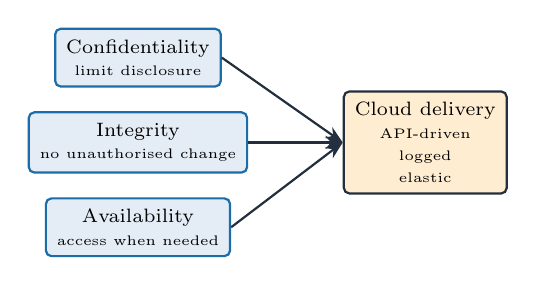
\begin{tikzpicture}[every node/.style={font=\scriptsize},node distance=3mm]
        \node[box,fill=accent!12] (c) {Confidentiality\\\tiny limit disclosure};
        \node[box,fill=accent!12,below=of c] (i) {Integrity\\\tiny no unauthorised change};
        \node[box,fill=accent!12,below=of i] (a) {Availability\\\tiny access when needed};
        \node[awsbox,right=12mm of i,fill=awsorange!18] (cloud)
          {Cloud delivery\\\tiny API-driven\\\tiny logged\\\tiny elastic};
        \draw[flow] (c.east) -- (cloud.west);
        \draw[flow] (i.east) -- (cloud.west);
        \draw[flow] (a.east) -- (cloud.west);
      \end{tikzpicture}}
    \end{column}
  \end{columns}
\end{frame}

\begin{frame}{AWS security objectives mapped to services}
  % Speaker note: this consolidates the original "Controllability/Auditability/..." slides.
  \centering\small
  \renewcommand{\arraystretch}{1.35}
  \begin{tabular}{>{\raggedright\arraybackslash}p{2.6cm} >{\raggedright\arraybackslash}p{6.3cm} l}
    \toprule
    \textbf{Objective} & \textbf{Question it answers} & \textbf{Primary service}\\
    \midrule
    Controllability & Who can act? temporary credentials? own keys? & \svc{IAM} / \svc{KMS}\\
    Auditability    & Who did what, when, from where?               & \svc{CloudTrail}\\
    Visibility      & What exists? what changed?                    & \svc{Config}\\
    Agility \& Automation & Reproducible, compliant deployments?    & \svc{CloudFormation}\\
    Threat detection & Anomalous / malicious behaviour?             & \svc{GuardDuty}\\
    \bottomrule
  \end{tabular}
  \vfill
  {\footnotesize\color{midgray}Each design principle below is realised by one or more of these services.}
\end{frame}

\begin{frame}{Seven security design principles (AWS Well-Architected)}
  \footnotesize
  \begin{columns}[T]
    \begin{column}{0.5\textwidth}
      \begin{enumerate}\setlength\itemsep{2pt}
        \item \term{Least privilege} --- grant as needed, separate duties, avoid long-term credentials.
        \item \term{Traceability} --- monitor, log, audit; alert and respond automatically.
        \item \term{Secure all layers} --- defence in depth across edge, VPC, subnet, instance, app, data.
        \item \term{Automate security} --- security as code, IaC, automated guardrails.
      \end{enumerate}
    \end{column}
    \begin{column}{0.5\textwidth}
      \begin{enumerate}\setlength\itemsep{2pt}\setcounter{enumi}{4}
        \item \term{Protect data in transit \& at rest} --- encrypt, classify, tokenise.
        \item \term{Keep people away from data} --- reduce direct access \& manual handling.
        \item \term{Prepare for security events} --- runbooks, game days, isolate \& recover.
      \end{enumerate}
      \vspace{0.5em}
      \begin{block}{\footnotesize MSc framing}
        \footnotesize These principles are the \emph{tactics}; \term{Zero Trust} (Part II.A) is the
        \emph{strategy} that ties them together.
      \end{block}
    \end{column}
  \end{columns}
\end{frame}

%==============================================================================
\section{Shared Responsibility Model}
%==============================================================================

\begin{frame}{Shared responsibility --- ``of the cloud'' vs.\ ``in the cloud''}
  \begin{columns}[T]
    \begin{column}{0.52\textwidth}\small
      \begin{itemize}
        \item \term{AWS} secures the infrastructure: hardware, global network, virtualisation,
              managed-service software --- ``security \emph{of} the cloud''.
        \item \term{Customer} secures configuration \& data: IAM, OS patching, SG/NACL rules,
              encryption, app logic --- ``security \emph{in} the cloud''.
        \item The line \term{moves with the service model}: the more managed, the more AWS owns.
      \end{itemize}
      \vspace{0.3em}
      {\footnotesize\color{midgray}Most real-world breaches sit on the \emph{customer} side:
      public S3 buckets, over-broad IAM, exposed instances.}
    \end{column}
    \begin{column}{0.48\textwidth}
      \centering
      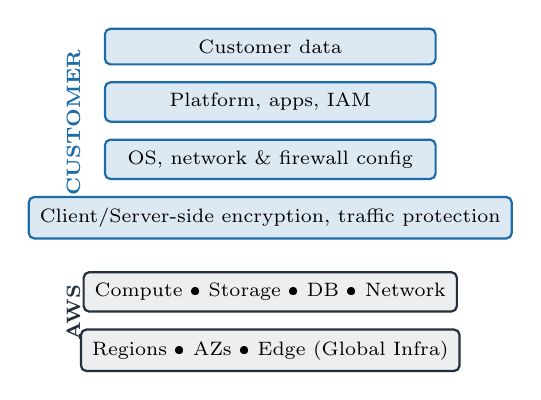
\begin{tikzpicture}[every node/.style={font=\scriptsize},node distance=2mm]
        \node[box,fill=accent!15,minimum width=4.2cm] (data) {Customer data};
        \node[box,fill=accent!15,minimum width=4.2cm,below=of data] (app)
          {Platform, apps, IAM};
        \node[box,fill=accent!15,minimum width=4.2cm,below=of app] (os)
          {OS, network \& firewall config};
        \node[box,fill=accent!15,minimum width=4.2cm,below=of os] (enc)
          {Client/Server-side encryption, traffic protection};
        \node[awsbox,minimum width=4.2cm,below=4mm of enc] (compute)
          {Compute \textbullet\ Storage \textbullet\ DB \textbullet\ Network};
        \node[awsbox,minimum width=4.2cm,below=of compute] (infra)
          {Regions \textbullet\ AZs \textbullet\ Edge (Global Infra)};
        \node[rotate=90,accent,font=\bfseries\scriptsize] at ([xshift=-2.5cm]app.south) {CUSTOMER};
        \node[rotate=90,awsink,font=\bfseries\scriptsize] at ([xshift=-2.5cm]compute.south) {AWS};
      \end{tikzpicture}
    \end{column}
  \end{columns}
\end{frame}

\begin{frame}{The boundary moves with the service model}
  \centering\small
  \renewcommand{\arraystretch}{1.25}
  \begin{tabular}{l l l}
    \toprule
    \textbf{Service} & \textbf{Customer owns} & \textbf{AWS owns}\\
    \midrule
    EC2 (IaaS)        & Guest OS, patching, SG, app, data, IAM & Hypervisor, host, network fabric\\
    RDS (PaaS)        & Schema, IAM, network, backups policy, data & DB engine patching, host OS\\
    S3 (storage)      & Bucket policy, ACL, encryption choice, data & Durability, infra, service software\\
    Lambda (serverless)& Code, IAM role, secrets, deps & Runtime, OS, scaling, patching\\
    EKS (managed K8s) & Worker nodes, RBAC, workloads, network policy & Control plane, etcd, API server\\
    \bottomrule
  \end{tabular}
  \vfill
  % Speaker note: EKS row foreshadows Part II.B (control-plane responsibility).
  {\footnotesize\color{midgray}Rule of thumb: the customer \emph{always} owns IAM, data classification,
  and ``who can access what''.}
\end{frame}

\begin{frame}{Exam-style question --- responsibility boundary}
  \begin{block}{Question}
    Under the shared responsibility model, who is responsible for configuring \term{security group rules}
    that decide which ports are open on an EC2 Linux instance?
  \end{block}
  \begin{columns}[T]
    \begin{column}{0.5\textwidth}\small
      \begin{enumerate}[A.]
        \item AWS configures the rules.
        \item \textbf{The customer configures the rules.}
        \item Security group rules are not needed.
        \item AWS configures rules; customer opens ports.
      \end{enumerate}
    \end{column}
    \begin{column}{0.5\textwidth}
      \begin{block}{\footnotesize Answer: B}
        \footnotesize Keyword: \emph{configuring security group rules}. SG configuration is always
        a customer responsibility (``in the cloud''), regardless of instance OS.
      \end{block}
    \end{column}
  \end{columns}
\end{frame}

%==============================================================================
\section{IAM \& Access Management}
%==============================================================================

\subsection{IAM fundamentals}

\begin{frame}{IAM: the control plane for ``who can do what''}
  \begin{columns}[T]
    \begin{column}{0.58\textwidth}\small
      \begin{itemize}
        \item \term{Authentication} --- establish the \emph{principal} (user, role, service)
              via credentials / federation / MFA.
        \item \term{Authorisation} --- evaluate \emph{policies} to allow or deny each request.
        \item A \term{request} carries: action, resource, principal, environment (IP, time, MFA),
              and resource data --- all usable in \term{conditions}.
      \end{itemize}
      \begin{block}{\footnotesize Building blocks}
        \footnotesize \term{User} (person/app) \textbullet\ \term{Group} (set of users) \textbullet\
        \term{Role} (assumable, temporary creds via STS) \textbullet\ \term{Policy} (JSON document).
      \end{block}
    \end{column}
    \begin{column}{0.42\textwidth}
      \centering
      \resizebox{\linewidth}{!}{%
      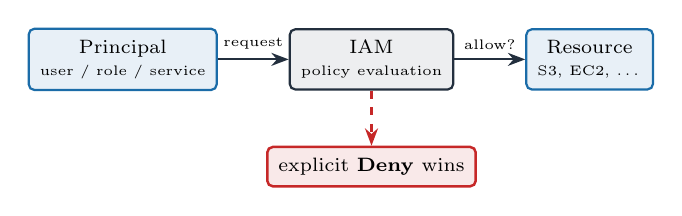
\begin{tikzpicture}[every node/.style={font=\scriptsize},node distance=5mm]
        \node[box] (user) {Principal\\\tiny user / role / service};
        \node[awsbox,right=9mm of user] (iam) {IAM\\\tiny policy evaluation};
        \node[box,right=9mm of iam] (res) {Resource\\\tiny S3, EC2, \dots};
        \draw[flow] (user) -- node[above,font=\tiny]{request} (iam);
        \draw[flow] (iam) -- node[above,font=\tiny]{allow?} (res);
        \node[hot,below=7mm of iam,minimum width=2.4cm] (deny)
          {explicit \textbf{Deny} wins};
        \draw[attack] (iam) -- (deny);
      \end{tikzpicture}}
    \end{column}
  \end{columns}
\end{frame}

\begin{frame}[fragile]{Policy evaluation logic --- the one rule to memorise}
  \begin{columns}[T]
    \begin{column}{0.5\textwidth}\small
      Effective permission = intersection of \emph{all} applicable policies:
      \begin{enumerate}\setlength\itemsep{1pt}
        \item Default: implicit \term{deny}.
        \item An \term{Allow} in any identity- or resource-based policy can grant access\dots
        \item \dots unless a \term{permissions boundary} / \term{Service Control Policy (SCP)} fails to allow it,
        \item \dots and an \term{explicit Deny anywhere always wins}.
      \end{enumerate}
      \vspace{0.4em}
      \begin{alertblock}{\footnotesize Common pitfall}
        \footnotesize A user with \texttt{Allow *} is still blocked if an SCP or boundary
        does not permit the action. Wildcards $\neq$ effective access.
      \end{alertblock}
    \end{column}
    \begin{column}{0.5\textwidth}
      \scriptsize\textbf{Identity-based} (attached to principal):
      \begin{lstlisting}
{ "Effect": "Allow",
  "Action": ["s3:GetObject"],
  "Resource": "arn:aws:s3:::reports/*",
  "Condition": {
    "Bool": {"aws:MultiFactorAuthPresent":"true"}
  } }
      \end{lstlisting}
      \textbf{Resource-based} (attached to resource): answers ``who can touch \emph{me}'',
      enables \term{cross-account} access without role assumption.

      \begin{block}{\footnotesize Service-Control Policy (SCP)}
        \footnotesize An organization-wide guardrail that sets the maximum permissions for AWS accounts. IAM permissions cannot exceed SCP limits.
       
       w IAM grants permissions; SCPs define the maximum permissions that can be granted.
      \end{block}
    \end{column}
    

  \end{columns}

\end{frame}

\begin{frame}{Guardrails: boundaries, SCPs, federation}
  \footnotesize
  \begin{columns}[T]
    \begin{column}{0.5\textwidth}
      \begin{itemize}
        \item \term{Permissions boundary} --- max permissions an identity \emph{can} be granted
              (e.g. team cannot delegate admin roles).
        \item \term{Service Control Policy (SCP)} --- org-wide ceiling across accounts
              (\svc{Organizations}); cannot grant, only limit.
        \item \term{Resource policy} --- access stated on the resource (S3 bucket policy, KMS key policy).
      \end{itemize}
    \end{column}
    \begin{column}{0.5\textwidth}
      \begin{itemize}
        \item \term{Federation} --- trust external IdP; no local users.
        \item \svc{IAM Identity Center} (ex-SSO) --- central, attribute-based, short-lived sessions.
        \item \svc{Cognito} --- identity for web/mobile apps.
        \item \svc{Directory Service} --- managed AD integration.
      \end{itemize}
      \begin{block}{\footnotesize SCP example}
        \scriptsize \texttt{Deny organizations:LeaveOrganization} on \texttt{"*"}
        --- member accounts cannot detach.
      \end{block}
    \end{column}
  \end{columns}
\end{frame}

\subsection{Modern IAM (Topic E)}

\begin{frame}{Modern IAM: from standing access to just-in-time}
  % Speaker note: this is extension topic E -- explicitly built on the IAM primitives above.
  \begin{columns}[T]
    \begin{column}{0.54\textwidth}\small
      \begin{itemize}
        \item \term{Temporary credentials by default} --- Security Token Service (STS) / roles / Identity Center sessions;
              kill long-lived access keys.
        \item \term{Just-in-Time (JIT) access} --- elevate only for an approved window, auto-revoke.
        \item \term{Privileged Access Management (PAM)} --- only allow time-boxed admin actions.
        \item \term{Break-glass accounts} --- only used if usual access fails; rarely-used, heavily-monitored, MFA-hardware,
              alarmed on every use.
        \item \term{Workload identity} --- machines get identity too: EC2 instance roles,
              IAM Roles for Service Accounts (IRSA) / Pod Identity (Part II.B), pods get access to AWS services without storing secrets in container.
      \end{itemize}
    \end{column}
    \begin{column}{0.46\textwidth}
      \begin{block}{\footnotesize Review \& detect drift}
        \footnotesize
        \svc{IAM Access Analyzer} --- finds resources shared externally; generates
        least-privilege policies from CloudTrail; validates policies.
      \end{block}
      \begin{block}{\footnotesize Cross-account access}
        \footnotesize Temporary role assumption rather than sharing secrets for cross-account access
        over sharing credentials.
      \end{block}
       \begin{block}{\footnotesize Security Token Service (STS)}
        \footnotesize STS creates temporarily valid tokens containing Access Key + Secret Key + Session Token; AWS services check token validity on each request% for own service: check e.g. via sts.get_caller_identity() API.
      \end{block}
      
    \end{column}
  \end{columns}
\end{frame}

\begin{frame}{IAM anti-patterns --- and the fix}
  \centering\small
  \renewcommand{\arraystretch}{1.3}
  \begin{tabular}{>{\raggedright\arraybackslash}p{5.2cm} >{\raggedright\arraybackslash}p{6.6cm}}
    \toprule
    \textbf{Anti-pattern \xmark} & \textbf{Mitigation \cmark}\\
    \midrule
    \texttt{Action:"*"} / \texttt{Resource:"*"} wildcards & Scope to actions+ARNs; generate policy from access history\\
    Long-lived access keys in code/CI & STS / IRSA / OIDC federation; Secrets Manager; rotation\\
    Shared / generic admin accounts & Per-identity federation; named principals in CloudTrail\\
    Standing admin privileges & JIT elevation + PAM + session recording\\
    \texttt{iam:PassRole} unscoped & Restrict which roles can be passed, to which service\\
    No boundary on delegated roles & Permissions boundaries + SCP ceiling\\
    \bottomrule
  \end{tabular}
  \vfill
  {\footnotesize\color{midgray}Almost every cloud breach report features at least two rows of this table.}
\end{frame}

%==============================================================================
\section{Infrastructure Security}
%==============================================================================

\begin{frame}{Network defence in depth: a three-tier web app}
  \centering
  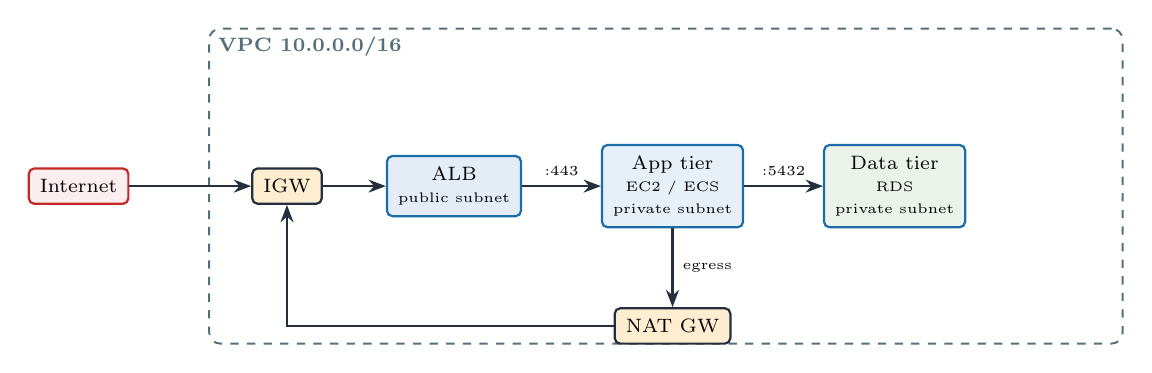
\begin{tikzpicture}[every node/.style={font=\scriptsize},node distance=6mm]
    % VPC boundary
    \node[zone,minimum width=11.6cm,minimum height=4.0cm] (vpc) {};
    \node[anchor=north west,font=\scriptsize\bfseries,midgray] at (vpc.north west) {VPC 10.0.0.0/16};
    % internet & igw
    \node[awsbox,left=10mm of vpc,fill=bad!8,draw=bad] (net) {Internet};
    \node[awsbox,fill=awsorange!18] (igw) at ([xshift=1.0cm]vpc.west) {IGW};
    % public subnet
    \node[box,right=8mm of igw,fill=accent!12] (alb) {ALB\\\tiny public subnet};
    % private app subnet
    \node[box,right=10mm of alb] (app) {App tier\\\tiny EC2 / ECS\\\tiny private subnet};
    % private data subnet
    \node[box,right=10mm of app,fill=good!10] (db) {Data tier\\\tiny RDS\\\tiny private subnet};
    \node[awsbox,below=10mm of app,fill=awsorange!18] (nat) {NAT GW};
    \draw[flow] (net) -- (igw);
    \draw[flow] (igw) -- (alb);
    \draw[flow] (alb) -- node[above,font=\tiny]{:443} (app);
    \draw[flow] (app) -- node[above,font=\tiny]{:5432} (db);
    \draw[flow] (app) -- node[right,font=\tiny]{egress} (nat);
    % return path routed along the bottom channel, clear of the ALB node
    \draw[flow] (nat.west) -| (igw.south);
  \end{tikzpicture}
  \vspace{0.4em}
  \begin{columns}[T]
    \begin{column}{0.5\textwidth}\footnotesize
      \begin{itemize}
        \item \term{Public subnet}: route to Internet Gateway (IGW); only the Application Load Balancer (ALB) is exposed.
        \item \term{Private subnets}: no inbound from internet; egress via NAT only.
      \end{itemize}
    \end{column}
    \begin{column}{0.5\textwidth}\footnotesize
      \begin{itemize}
        \item Layers: IGW $\to$ Network Access Control List (NACL) $\to$ Security Group $\to$ host firewall $\to$ app.
        \item DB tier reachable \emph{only} from the app-tier security group.
      \end{itemize}
    \end{column}
  \end{columns}
\end{frame}

\begin{frame}{Security Groups vs.\ Network ACLs}
  \centering\small
  \renewcommand{\arraystretch}{1.3}
  \begin{tabular}{l l l}
    \toprule
    \textbf{Attribute} & \textbf{Security Group} & \textbf{Network ACL}\\
    \midrule
    Scope        & Instance / Elastic Network Interface (ENI) level            & Subnet level\\
    Rules        & Allow only                      & Allow \emph{and} Deny\\
    State        & Stateful (return traffic auto)  & Stateless (must allow return)\\
    Evaluation   & All rules evaluated together    & Lowest rule number first\\
    Typical use  & Primary instance firewall       & Coarse subnet guardrail, block bad IPs\\
    \bottomrule
  \end{tabular}
  \vfill
  \begin{columns}[T]
    \begin{column}{0.5\textwidth}\footnotesize
      \begin{block}{\footnotesize Good SG practice}
        \footnotesize Reference \emph{other security groups} as sources, not CIDRs ---
        tiers authorise tiers, addresses can change.
      \end{block}
    \end{column}
    \begin{column}{0.5\textwidth}\footnotesize
      \begin{itemize}
        \item Also in the VPC toolbox: \term{route tables}, \term{VPC endpoints}
              (private S3/KMS access), \term{VPC Flow Logs} (Sec.~6).
        \item \term{Limit exposure}: no ('not allow') \texttt{0.0.0.0/0} on :22/:3389.
      \end{itemize}
    \end{column}
  \end{columns}
\end{frame}

%==============================================================================
\section{Data Protection}
%==============================================================================

\begin{frame}{Protecting data at rest --- S3 first, because that is where it leaks}
  \begin{columns}[T]
    \begin{column}{0.55\textwidth}\small
      \begin{itemize}
        \item Objects are private by default --- leaks come from \term{misconfiguration}.
        \item \term{S3 Block Public Access} --- account/bucket-level kill switch for public ACLs \& policies.
        \item \term{Versioning} (+ MFA delete) --- recover from deletion/ransomware.
        \item \term{Object Lock} (Write Once, Read Many (WORM), governance/compliance) --- immutability for audit logs.
        \item Access = identity-based $\cap$ resource (bucket) policy; explicit deny wins.
      \end{itemize}
    \end{column}
    \begin{column}{0.45\textwidth}
      \begin{alertblock}{\footnotesize Classic breach pattern}
        \footnotesize Public bucket + sensitive objects + no logging $\Rightarrow$ silent mass
        exfiltration. Detect with \svc{Macie} + \svc{Config}; threat-model in Part II.D.
      \end{alertblock}
      \begin{block}{\footnotesize Defaults to enforce}
        \footnotesize Block Public Access \emph{on}, default encryption \emph{on},
        versioning \emph{on}, access logging \emph{on}.
      \end{block}
    \end{column}
  \end{columns}
\end{frame}

\begin{frame}{Encryption: client-side vs.\ server-side, and KMS}
  \begin{columns}[T]
    \begin{column}{0.5\textwidth}\small
      \begin{itemize}
        \item \term{Client-Side Encryption (CSE)} --- you encrypt before upload; AWS never sees plaintext or keys.
        \item \term{Server-Side Encryption (SSE)} --- AWS encrypts after receipt; transparent. Variants:
          \begin{itemize}
            \item \term{SSE-S3} --- AWS-managed keys.
            \item \term{SSE-KMS} --- KMS keys, \emph{envelope encryption}, policy + audit.
            \item \term{SSE-C} --- you supply keys per request.
          \end{itemize}
        \item In transit: \term{TLS} everywhere; \svc{AWS Certificate Manager (ACM)} issues/rotates certs; VPC endpoints
              keep traffic off the public internet.
      \end{itemize}
    \end{column}
    \begin{column}{0.5\textwidth}
      \centering
      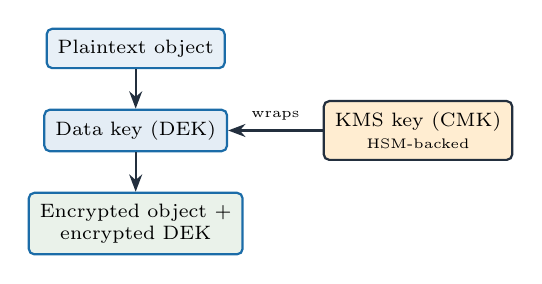
\begin{tikzpicture}[every node/.style={font=\scriptsize},node distance=5mm]
        \node[box] (data) {Plaintext object};
        \node[box,below=of data,fill=accent!12] (dek) {Data key (DEK)};
        \node[awsbox,right=12mm of dek,fill=awsorange!18] (cmk) {KMS key (CMK)\\\tiny HSM-backed};
        \node[box,below=of dek,fill=good!10] (enc) {Encrypted object +\\ encrypted DEK};
        \draw[flow] (data) -- (dek);
        \draw[flow] (cmk) -- node[above,font=\tiny]{wraps} (dek);
        \draw[flow] (dek) -- (enc);
      \end{tikzpicture}
      \\[0.3em]
      {\scriptsize Envelope encryption: KMS protects the DEK; usage is policy-controlled \& logged in CloudTrail.}
    \begin{block}{Cryptographic details}
      $\text{DEK} \leftarrow \text{random}(256 \text{ bit})$ 
    $\text{Ciphertext} = \text{AES}(\text{DEK}, \text{Daten})$ 

    $\text{Wrapped\_DEK} = \text{AES}(\text{KMS\_Key}, \text{DEK})$ 
    \end{block}
      
    \end{column}
    
      
    

  \end{columns}
  % Speaker note: tie KMS key policy back to "resource-based policy" from the IAM section.
\end{frame}

\begin{frame}{Secrets, classification \& data-layer services}
  \footnotesize
  \begin{columns}[T]
    \begin{column}{0.5\textwidth}
      \begin{itemize}
        \item \svc{Secrets Manager} --- store/rotate DB creds, API keys; no secrets in code/config.
        \item \svc{KMS} --- centralised key lifecycle \& usage policy.
        \item \svc{ACM} (+ Private CA) --- TLS certificate lifecycle.
      \end{itemize}
    \end{column}
    \begin{column}{0.5\textwidth}
      \begin{itemize}
        \item \svc{Macie} --- discover \& classify PII in S3; flag public/unencrypted/shared buckets.
        \item \term{Presigned URLs} --- time-boxed, scoped object access without IAM users.
        \item \term{Least privilege} on data: enforce encryption on every PUT.
      \end{itemize}
    \end{column}
  \end{columns}
  \vfill
  \begin{block}{\footnotesize Presigned URL}
    \footnotesize A URL with embedded temporary credentials that grants access to a specific S3 object for a limited time, without needing an IAM user or role.
    
    

  \end{block}
\end{frame}

%==============================================================================
\section{Logging \& Monitoring}
%==============================================================================

\begin{frame}{Capture everything: the cloud audit substrate}
  \begin{columns}[T]
    \begin{column}{0.5\textwidth}\small
      \begin{itemize}
        \item \svc{CloudTrail} --- \emph{who did what, when, from where} (API audit).
              The single most important security log.
        \item \svc{CloudWatch} --- metrics, logs, alarms, dashboards (operational health).
        \item \svc{Config} --- resource inventory + configuration history + rule evaluation
              (``what exists / what changed'').
        \item \svc{EventBridge} --- event bus that routes signals to automated responders.
      \end{itemize}
    \end{column}
    \begin{column}{0.5\textwidth}\small
      \begin{block}{\footnotesize Built-in service logs}
        \footnotesize \term{VPC Flow Logs} (network), \term{S3 server access logs},
        \term{ELB access logs}, \term{DNS / Route\,53 logs}.
      \end{block}
      \begin{block}{\footnotesize CloudTrail vs.\ CloudWatch}
        \footnotesize CloudTrail = \emph{accountability} (who/what); CloudWatch = \emph{behaviour}
        (anomaly/alarm). Combine: CloudTrail event $\to$ EventBridge rule $\to$ alarm/automation.
      \end{block}
      \begin{block}{\footnotesize EventBridge vs. SQS}
        \footnotesize SQS: like mailbox, pull-based; EventBridge: like pub/sub, push-based. EventBridge for real-time, SQS for decoupling.
      \end{block}
    \end{column}
  \end{columns}
\end{frame}

\begin{frame}{Posture management \& aggregation}
  \footnotesize
  \begin{itemize}
    \item \svc{Security Hub} --- aggregates findings (GuardDuty, Inspector, Macie, partners) into
          one normalised view + best-practice standards scoring.
    \item \svc{Config} rules --- continuous compliance (e.g.\ ``no public S3'', ``encryption on'',
          ``no \texttt{0.0.0.0/0} SSH'') with auto-remediation hooks.
    \item \svc{Trusted Advisor} --- account-wide best-practice checks.
  \end{itemize}
  \vfill
  \begin{exampleblock}{\footnotesize Reading a CloudTrail event (key fields)}
    \scriptsize \texttt{userIdentity} (who) \textbullet\ \texttt{eventName} (what, e.g.\ \texttt{StopInstances})
    \textbullet\ \texttt{eventTime}, \texttt{sourceIPAddress}, \texttt{userAgent} (when/where)
    \textbullet\ \texttt{requestParameters} / \texttt{responseElements} (detail).
  \end{exampleblock}
  \begin{block}{\footnotesize Equivalences}
    \footnotesize SIEM $\approx$ CloudTrail + CloudWatch + Logs\\
    \footnotesize SOAR $\approx$ EventBridge + Lambda/Step Functions \\
    \footnotesize Security Hub + Config rules $\approx$ vulnerability management / posture management platform
  \end{block}
  % Speaker note: these fields become the detection signals in Part II.F.
\end{frame}

%==============================================================================
\section{Incident Response}
%==============================================================================

\begin{frame}{IR in the cloud: phases \& supporting services}
  \centering
  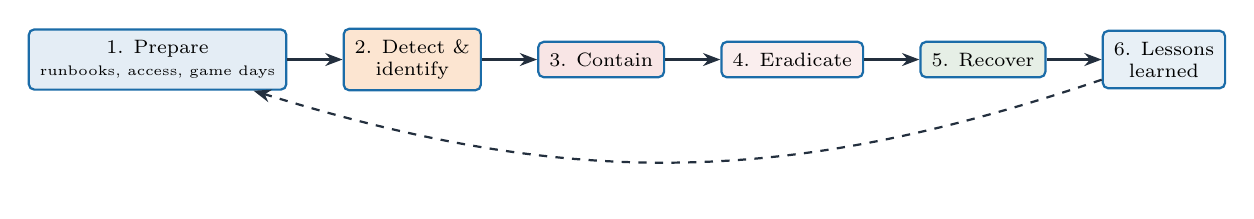
\begin{tikzpicture}[every node/.style={font=\scriptsize},node distance=7mm]
    \node[box,fill=accent!12] (p1) {1. Prepare\\\tiny runbooks, access, game days};
    \node[box,right=of p1,fill=warn!18] (p2) {2. Detect \&\\identify};
    \node[box,right=of p2,fill=bad!12] (p3) {3. Contain};
    \node[box,right=of p3,fill=bad!8] (p4) {4. Eradicate};
    \node[box,right=of p4,fill=good!12] (p5) {5. Recover};
    \node[box,right=of p5,fill=accent!10] (p6) {6. Lessons\\learned};
    \draw[flow] (p1)--(p2); \draw[flow] (p2)--(p3); \draw[flow] (p3)--(p4);
    \draw[flow] (p4)--(p5); \draw[flow] (p5)--(p6);
    \draw[flow,dashed] (p6) to[bend left=18] (p1);
  \end{tikzpicture}
  \vspace{0.6em}
  \begin{columns}[T]
    \begin{column}{0.5\textwidth}\footnotesize
      \textbf{Discovery / recognition}
      \begin{itemize}
        \item \svc{GuardDuty} (threat detection), \svc{Inspector} (vulns),
              \svc{Config} (drift), \svc{CloudWatch}, \svc{Shield} (DDoS).
      \end{itemize}
    \end{column}
    \begin{column}{0.5\textwidth}\footnotesize
      \textbf{Resolution / recovery}
      \begin{itemize}
        \item \svc{Systems Manager} (act on fleet), \svc{CloudFormation}
              (rebuild forensic VPC), \svc{Lambda}/\svc{Step Functions}/\svc{SNS}
              (event-driven automation).
      \end{itemize}
    \end{column}
  \end{columns}
\end{frame}

\begin{frame}{IR best practices --- and why automation matters}
  \begin{columns}[T]
    \begin{column}{0.55\textwidth}\small
      \begin{itemize}
        \item Identify key people, external resources, tooling \emph{before} the incident.
        \item \term{Pre-provision} break-glass access \& forensic tooling.
        \item \term{Automate containment} --- isolate an instance/role in seconds, not hours.
        \item Write \term{runbooks}; rehearse with \term{game days} in a safe environment.
        \item Capture evidence \emph{before} you terminate (snapshots, memory, logs).
      \end{itemize}
    \end{column}
    \begin{column}{0.45\textwidth}
      \begin{block}{\footnotesize Cloud advantage}
        \footnotesize Compromised host? Don't clean it --- \term{isolate, snapshot, redeploy from IaC}.
        Immutable infrastructure makes eradication a re-deploy.
      \end{block}
      \begin{block}{\footnotesize Forward link}
        \footnotesize Part II.F turns these phases into four concrete, event-driven
        \term{playbooks}.
      \end{block}
    \end{column}
  \end{columns}
\end{frame}

%##############################################################################
%  PART II -- ADVANCED CLOUD SECURITY (MASTER EXTENSIONS)
%##############################################################################

\begin{frame}[plain,noframenumbering]
  \vfill\centering
  {\color{awsorange}\rule{0.25\paperwidth}{2.5pt}}\\[0.8em]
  {\usebeamerfont{title}\color{awsink}Part II}\\[0.4em]
  {\Large\color{awsink}Advanced Cloud Security}\\[0.6em]
  {\color{midgray}\small Zero Trust \textbullet\ Containers/Kubernetes \textbullet\ Supply Chain
   \textbullet\ Threat Modeling \textbullet\ Detection \& Response}\\[0.8em]
  {\footnotesize\color{midgray}Each topic is connected back to the AWS controls from Part I.}
  \vfill
\end{frame}

%==============================================================================
\section{A. Zero Trust in Cloud Environments}
%==============================================================================

\begin{frame}{Zero Trust: never trust, always verify}
  \begin{columns}[T]
    \begin{column}{0.56\textwidth}\small
      \begin{itemize}
        \item \term{Core principle}: no implicit trust from network location ---
              \emph{every} request is authenticated, authorised \& encrypted.
        \item \term{Identity is the new perimeter} --- controls follow the principal
              (user \emph{and} workload), not the IP subnet.
        \item \term{Continuous verification} --- trust is re-evaluated per request using
              identity, device/workload posture, and context (time, geo, risk).
        \item \term{Assume breach} --- minimise blast radius via least privilege \& segmentation.
      \end{itemize}
      {\footnotesize\color{midgray}Reference model: NIST SP\,800-207.}
    \end{column}
    \begin{column}{0.44\textwidth}
      \centering
      \resizebox{\linewidth}{!}{%
      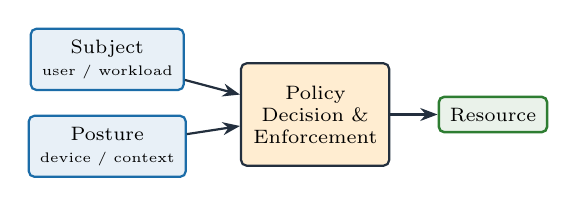
\begin{tikzpicture}[every node/.style={font=\scriptsize},node distance=3mm]
        \node[box] (subj) {Subject\\\tiny user / workload};
        \node[box,below=of subj] (dev) {Posture\\\tiny device / context};
        \node[awsbox,right=7mm of subj,yshift=-7mm,fill=awsorange!18,minimum height=1.3cm,
              text width=1.6cm] (pep) {Policy\\Decision \&\\Enforcement};
        \node[ok,right=6mm of pep] (res) {Resource};
        \draw[flow] (subj) -- (pep); \draw[flow] (dev) -- (pep);
        \draw[flow] (pep) -- (res);
      \end{tikzpicture}}
      \\[0.3em]{\scriptsize\color{midgray}Trust re-evaluated on \emph{every} request.}
    \end{column}
  \end{columns}
\end{frame}

\begin{frame}{Perimeter-based vs.\ Zero Trust}
  \centering\small
  \renewcommand{\arraystretch}{1.3}
  \begin{tabular}{>{\raggedright\arraybackslash}p{3.0cm} >{\raggedright\arraybackslash}p{4.7cm} >{\raggedright\arraybackslash}p{4.7cm}}
    \toprule
     & \textbf{Classic perimeter} & \textbf{Zero Trust}\\
    \midrule
    Trust anchor   & Network location (``inside = trusted'') & Verified identity + context\\
    Default stance & Allow within perimeter                  & Deny; allow per verified request\\
    Lateral movement& Easy once inside                       & Contained by segmentation\\
    Enforcement    & Firewall at the edge                    & Distributed, per-resource\\
    Credentials    & Often long-lived                        & Short-lived, continuously re-checked\\
    \bottomrule
  \end{tabular}
  \vfill
  \begin{alertblock}{\footnotesize Why the cloud forces this}
    \footnotesize There is no single edge to defend: APIs are internet-reachable, workloads are
    ephemeral, identities are many. The ``castle wall'' dissolves.
  \end{alertblock}
\end{frame}

\begin{frame}{Zero Trust pillars realised with existing AWS controls}
  \centering\small
  \renewcommand{\arraystretch}{1.3}
  \begin{tabular}{>{\raggedright\arraybackslash}p{4.2cm} >{\raggedright\arraybackslash}p{7.4cm}}
    \toprule
    \textbf{Zero Trust pillar} & \textbf{AWS realisation (from Part I)}\\
    \midrule
    Strong identity, least privilege & \svc{IAM} roles, permissions boundaries, SCPs; STS short-lived creds\\
    Continuous verification / audit  & \svc{CloudTrail} (every API call) + \svc{Config} (state) + conditions\\
    Micro-segmentation               & \svc{Security Groups} (SG-references-SG), private subnets, \svc{VPC} endpoints\\
    Workload identity                & EC2 instance roles, EKS \term{IRSA} / Pod Identity (Sec.~B)\\
    Encryption everywhere            & TLS in transit, \svc{KMS} at rest --- no plaintext on the wire\\
    Adaptive / risk signals          & \svc{GuardDuty} findings feeding policy / response (Sec.~F)\\
    \bottomrule
  \end{tabular}
  \vfill
  \bridge{Zero Trust is not a product to buy --- it is how you \emph{compose} IAM, VPC, SG,
  CloudTrail and Config. The MFA \texttt{Condition} and SG-references-SG patterns you already saw
  are Zero Trust in practice.}
\end{frame}

%==============================================================================
\section{B. Container \& Kubernetes Security}
%==============================================================================

\begin{frame}{Container threat model: where the attack surface lives}
  \centering
  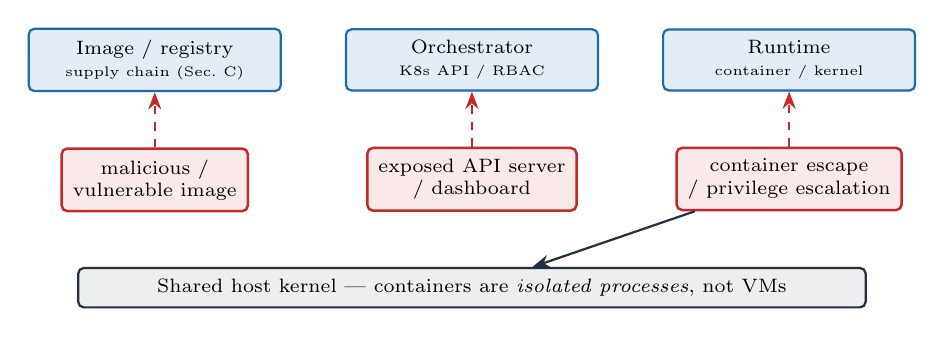
\begin{tikzpicture}[every node/.style={font=\scriptsize},node distance=3.5mm]
    \node[box,fill=accent!12,minimum width=3.2cm] (img) {Image / registry\\\tiny supply chain (Sec.~C)};
    \node[box,fill=accent!12,minimum width=3.2cm,right=8mm of img] (orch) {Orchestrator\\\tiny K8s API / RBAC};
    \node[box,fill=accent!12,minimum width=3.2cm,right=8mm of orch] (run) {Runtime\\\tiny container / kernel};
    \node[hot,below=7mm of img] (a1) {malicious /\\vulnerable image};
    \node[hot,below=7mm of orch] (a2) {exposed API server\\/ dashboard};
    \node[hot,below=7mm of run] (a3) {container escape\\/ privilege escalation};
    \draw[attack] (a1) -- (img); \draw[attack] (a2) -- (orch); \draw[attack] (a3) -- (run);
    \node[awsbox,fill=awsink!8,below=7mm of a2,minimum width=10cm] (host)
      {Shared host kernel --- containers are \emph{isolated processes}, not VMs};
    \draw[flow] (a3) -- (host);
  \end{tikzpicture}
  \vspace{0.4em}
  \begin{itemize}\footnotesize
    \item Containers share the host kernel $\Rightarrow$ a kernel/runtime escape breaks isolation.
    \item Four control points: \term{image}, \term{registry}, \term{orchestrator}, \term{runtime}
          --- secure all four (defence in depth).
  \end{itemize}
  \begin{block}{\footnotesize Container Escape}
    \footnotesize Container escape, e.g. via kernel vulnerabilities (patching!), over-privileged containers, host file system is mounted, Linux too many capabilities, runtime weaknesses. Mitigate with least privilege, seccomp/AppArmor, no privileged containers, runtime detection (Falco).
  \end{block}
\end{frame}

\begin{frame}{Kubernetes security building blocks}
  \footnotesize
  \begin{columns}[T]
    \begin{column}{0.5\textwidth}
      \begin{itemize}
        \item \term{RBAC} --- bind subjects (users, groups, service accounts) to verbs on resources;
              least privilege at the API.
        \item \term{Service Accounts} --- workload identity inside the cluster; do \emph{not} auto-mount
              tokens you don't need.
        \item \term{Admission control} --- validate/mutate objects at create time
              (e.g.\ OPA/Gatekeeper, Kyverno, Pod Security Admission).
        \item \term{Network Policies} --- default-deny pod-to-pod; the SG/NACL analogue inside the cluster.
      \end{itemize}
    \end{column}
    \begin{column}{0.5\textwidth}
      \begin{itemize}
        \item \term{Secrets} --- avoid plaintext in manifests; integrate KMS / external secret stores;
              encrypt etcd at rest.
        \item \term{Runtime security} --- detect anomalous syscalls/process behaviour
              (e.g.\ Falco), enforce seccomp/AppArmor.
        \item \term{Image security} --- scan, pin digests, use minimal/distroless bases (Sec.~C).
      \end{itemize}
      \begin{block}{\footnotesize Mental model}
        \footnotesize RBAC $\approx$ IAM, NetworkPolicy $\approx$ Security Group,
        Admission $\approx$ Config rule / SCP guardrail.
      \end{block}
    \end{column}
  \end{columns}
\end{frame}

\begin{frame}[fragile]{EKS specifics: who owns what, and workload identity}
  \begin{columns}[T]
    \begin{column}{0.52\textwidth}\small
      \begin{itemize}
        \item \term{Control-plane responsibility}: AWS runs/patches the API server \& etcd;
              \emph{you} own worker nodes, RBAC, workloads, network policy.
        \item \term{IRSA} (IAM Roles for Service Accounts) --- map a K8s service account to an IAM role
              via OIDC; pods get \term{scoped, short-lived} AWS credentials.
        \item \term{EKS Pod Identity} --- newer, simpler association of IAM roles to pods.
        \item Result: \emph{no static AWS keys in containers} --- workload identity, Zero Trust style.
      \end{itemize}
    \end{column}
    \begin{column}{0.48\textwidth}
      \scriptsize\textbf{RBAC: read-only pods, one namespace}
      \begin{lstlisting}
kind: Role
apiVersion: rbac.authorization.k8s.io/v1
metadata: { namespace: payments }
rules:
- apiGroups: [""]
  resources: ["pods"]
  verbs: ["get","list","watch"]   # no create/delete
      \end{lstlisting}
      \bridge{\scriptsize EKS extends the shared responsibility model: control plane = AWS,
      data plane = you. IRSA reuses IAM + STS from Part I.}
    \end{column}
  \end{columns}
\end{frame}

\begin{frame}{Typical attacks $\rightarrow$ best-practice mitigations}
  \centering\small
  \renewcommand{\arraystretch}{1.3}
  \begin{tabular}{>{\raggedright\arraybackslash}p{5.6cm} >{\raggedright\arraybackslash}p{6.2cm}}
    \toprule
    \textbf{Attack \xmark} & \textbf{Mitigation \cmark}\\
    \midrule
    Malicious / vulnerable image & Scan in CI \& registry; pin digests; signed images (Sec.~C)\\
    Exposed dashboard / API server & No public API endpoint; authn+RBAC; network policy; admission\\
    Privilege escalation in cluster & Least-privilege RBAC; no \texttt{cluster-admin} bindings; PSA\\
    Container escape & Non-root + read-only rootfs; drop caps; seccomp/AppArmor; no privileged pods\\
    Credential theft from pod & IRSA/Pod Identity (no static keys); short-lived tokens\\
    Resource exhaustion / crypto-mining & Resource \texttt{limits}/quotas; runtime detection (Falco)\\
    \bottomrule
  \end{tabular}
  \vfill
  {\footnotesize\color{midgray}Baseline hardening: minimal images, non-root, read-only filesystem,
  dropped capabilities, resource limits, image scanning.}
\end{frame}

%==============================================================================
\section{C. Supply Chain Security}
%==============================================================================

\begin{frame}{CI/CD is production access --- and a prime attack surface}
  \centering
  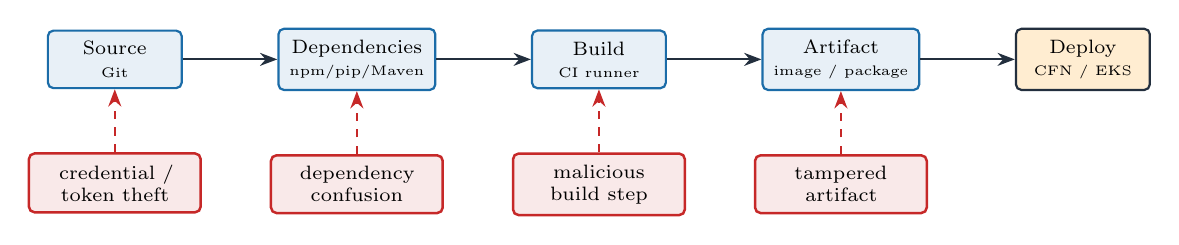
\begin{tikzpicture}[every node/.style={font=\scriptsize},node distance=12mm,
                      hot/.append style={text width=1.9cm,align=center}]
    \node[box,minimum width=1.7cm] (src) {Source\\\tiny Git};
    \node[box,minimum width=1.7cm,right=of src] (dep) {Dependencies\\\tiny npm/pip/Maven};
    \node[box,minimum width=1.7cm,right=of dep] (build) {Build\\\tiny CI runner};
    \node[box,minimum width=1.7cm,right=of build] (art) {Artifact\\\tiny image / package};
    \node[awsbox,minimum width=1.7cm,right=of art,fill=awsorange!18] (deploy) {Deploy\\\tiny CFN / EKS};
    \draw[flow] (src)--(dep); \draw[flow] (dep)--(build);
    \draw[flow] (build)--(art); \draw[flow] (art)--(deploy);
    % attack points (illustrative)
    \node[hot,below=8mm of src] (h1) {credential /\\token theft};
    \node[hot,below=8mm of dep] (h2) {dependency\\confusion};
    \node[hot,below=8mm of build] (h3) {malicious\\build step};
    \node[hot,below=8mm of art] (h4) {tampered\\artifact};
    \draw[attack] (h1)--(src); \draw[attack] (h2)--(dep);
    \draw[attack] (h3)--(build); \draw[attack] (h4)--(art);
  \end{tikzpicture}
  \vspace{0.3em}
  \begin{itemize}\footnotesize
    \item A pipeline with deploy rights is a privileged identity --- treat its credentials accordingly.
    \item Trust must be \term{verifiable end-to-end}: source $\to$ build $\to$ artifact $\to$ deploy.
  \end{itemize}
\end{frame}

\begin{frame}{Threats \& defences across the chain}
  \begin{columns}[T]
    \begin{column}{0.48\textwidth}
      \small\textbf{\color{bad}Threats}
      \begin{itemize}\footnotesize
        \item \term{Dependency confusion} --- internal package name resolves to attacker's public package.
        \item \term{Compromised packages} --- typosquatting, hijacked maintainer, malicious update.
        \item \term{Malicious build steps} --- poisoned CI config, compromised runner/plugin.
        \item \term{Secrets in pipelines} --- tokens in logs, env vars, or committed files.
        \item \term{Tampered artifacts} --- swapped image between build and deploy.
      \end{itemize}
    \end{column}
    \begin{column}{0.52\textwidth}
      \small\textbf{\color{good}Defences}
      \begin{itemize}\footnotesize
        \item \term{Software Bill of Materials (SBOM)} --- inventory every component (CycloneDX/SPDX); track with Dependency-Track.
        \item \term{Signing \& verification} --- sign commits, artifacts, images (Sigstore/cosign);
              verify at admission.
        \item \term{Provenance \& Supply-chain Levels for Software Artifacts (SLSA)} --- attest \emph{how/where} an artifact was built; raise SLSA level.
        \item \term{Reproducible builds} --- same input $\Rightarrow$ same output (detect tampering).
        \item \term{Policy-as-Code} --- gate deploys on scan/sign/provenance checks (OPA/Kyverno).
        \item \term{Secrets hygiene} --- OIDC to cloud, no long-lived keys; scoped, ephemeral tokens.
      \end{itemize}
    \end{column}
  \end{columns}
\end{frame}

\begin{frame}{Anchoring supply-chain controls in AWS}
  \footnotesize
  \begin{itemize}
    \item \term{Image signing/verification} --- sign in CI, store in \svc{ECR}, verify with an
          \term{admission controller} on EKS before a pod runs.
    \item \term{IaC integrity} --- \svc{CloudFormation}/Terraform reviewed, scanned (cfn-guard, checkov),
          and policy-gated; drift caught by \svc{Config}.
    \item \term{Pipeline identity} --- \svc{GitHub Actions}/\svc{GitLab CI} authenticate to AWS via
          \term{OIDC} $\to$ short-lived role, never stored access keys.
    \item \term{Secret detection} --- scan repos/pipelines; route findings to the
          ``exposed secret'' playbook (Sec.~F).
    \item \term{Vulnerability scanning} --- \svc{Inspector} scans ECR images continuously.
  \end{itemize}
  \vfill
  \bridge{The pipeline becomes a Zero-Trust principal: it proves its identity (OIDC), gets
  least-privilege short-lived credentials, and every artifact it produces is signed \& attested.}
  % Speaker note: emphasise OIDC federation replacing long-lived CI keys -- ties to Modern IAM (E).
\end{frame}

%==============================================================================
\section{D. Threat Modeling for Cloud Architectures}
%==============================================================================

\begin{frame}{Threat modeling: structure the question ``what can go wrong?''}
  \begin{columns}[T]
    \begin{column}{0.5\textwidth}\small
      Four guiding questions (Shostack):
      \begin{enumerate}\setlength\itemsep{1pt}
        \item What are we building? (\term{assets, data flows})
        \item What can go wrong? (\term{threats})
        \item What will we do about it? (\term{mitigations})
        \item Did we do a good job? (\term{validate})
      \end{enumerate}
      \vspace{0.3em}
      Identify: \term{assets}, \term{trust boundaries}, \term{entry points},
      \term{data flows}.
    \end{column}
    \begin{column}{0.5\textwidth}
      \centering\scriptsize\textbf{STRIDE for cloud}
      \renewcommand{\arraystretch}{1.15}
      \begin{tabular}{l l}
        \toprule
        \textbf{Threat} & \textbf{Cloud example}\\
        \midrule
        Spoofing        & Stolen IAM keys, assumed role\\
        Tampering       & Modified S3 object, poisoned image\\
        Repudiation     & CloudTrail disabled, no logs\\
        Info disclosure & Public bucket, unencrypted traffic\\
        Denial of service& Resource exhaustion, no quotas\\
        Elevation of priv& Over-broad IAM, \texttt{PassRole}\\
        \bottomrule
      \end{tabular}
    \end{column}
  \end{columns}
\end{frame}

% \begin{frame}{Worked example: three-tier web app in AWS}
%   \centering
%   \begin{tikzpicture}[every node/.style={font=\scriptsize},node distance=8mm]
%     \node[awsbox,fill=bad!8,draw=bad] (user) {Internet user};
%     \node[zone,minimum width=10.5cm,minimum height=2.6cm,right=6mm of user] (vpc) {};
%     \node[anchor=north west,font=\tiny\bfseries,midgray] at (vpc.north west) {Trust boundary: VPC};
%     \node[box,fill=accent!12] (alb) at ([xshift=-3.4cm]vpc.center) {ALB\\\tiny TLS};
%     \node[box,right=10mm of alb] (ec2) {EC2 app};
%     \node[box,fill=good!10,right=10mm of ec2] (rds) {RDS};
%     \node[awsbox,below=10mm of ec2,fill=awsorange!12] (s3) {S3 bucket};
%     \draw[flow] (user) -- (alb);
%     \draw[flow] (alb) -- (ec2); \draw[flow] (ec2) -- (rds); \draw[flow] (ec2) -- (s3);
%     % threat callouts
%     \node[hot,above=2mm of alb,font=\tiny] {(T) unencrypted\\traffic};
%     \node[hot,above=2mm of rds,font=\tiny] {(I) over-broad\\IAM role};
%     \node[hot,below=2mm of s3,font=\tiny] {(I) public\\bucket};
%     \node[hot,below=2mm of ec2,xshift=-2.2cm,font=\tiny] {(E) exposed\\EC2 / SSH};
%   \end{tikzpicture}
%   \vspace{0.3em}
%   \begin{itemize}\footnotesize
%     \item Threats to enumerate: public S3 bucket, overly-permissive IAM role, exposed EC2,
%           \term{lateral movement} app$\to$DB, unencrypted traffic, weak logging.
%     \item Each maps to a Part-I control: Block Public Access, least-privilege IAM, SG, TLS/KMS, CloudTrail.
%   \end{itemize}
% \end{frame}

\begin{frame}{A repeatable threat-modeling workflow}
  \centering
  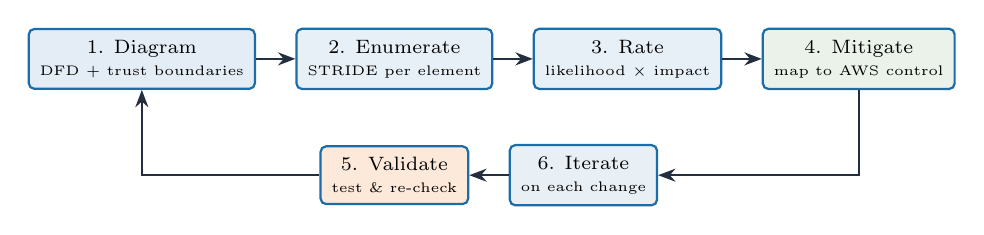
\begin{tikzpicture}[every node/.style={font=\scriptsize},node distance=5mm]
    \node[box,fill=accent!12] (s1) {1. Diagram\\\tiny DFD + trust boundaries};
    \node[box,right=of s1] (s2) {2. Enumerate\\\tiny STRIDE per element};
    \node[box,right=of s2] (s3) {3. Rate\\\tiny likelihood $\times$ impact};
    \node[box,right=of s3,fill=good!10] (s4) {4. Mitigate\\\tiny map to AWS control};
    \node[box,below=7mm of s2,fill=warn!15] (s5) {5. Validate\\\tiny test \& re-check};
    \node[box,right=of s5,fill=accent!10] (s6) {6. Iterate\\\tiny on each change};
    \draw[flow] (s1)--(s2); \draw[flow] (s2)--(s3); \draw[flow] (s3)--(s4);
    \draw[flow] (s4) |- (s6); \draw[flow] (s6)--(s5); \draw[flow] (s5) -| (s1);
  \end{tikzpicture}
  \vspace{0.6em}
  \begin{itemize}\footnotesize
    \item Do it \term{early} (design) and \term{continuously} (every architecture change /
          new entry point).
    \item Output is a living artifact: threats $\to$ owners $\to$ controls $\to$ verification status.
    \item Pair with \svc{Config} rules so mitigations are \term{enforced}, not just documented.
  \end{itemize}
\end{frame}

\begin{frame}{Exercise --- ``Identify threats and mitigations''}
  \begin{exampleblock}{Scenario}
    \small A startup deploys: a public \svc{ALB} $\to$ \svc{EC2} app (role allows \texttt{s3:*})
    $\to$ \svc{RDS}. Static files live in an \svc{S3} bucket with ACL ``public-read''. SSH (:22) is
    open to \texttt{0.0.0.0/0}. CloudTrail is \emph{not} enabled. Secrets sit in an EC2 user-data script.
  \end{exampleblock}
  \begin{columns}[T]
    \begin{column}{0.5\textwidth}\small
      \textbf{Task (15 min, in pairs)}
      \begin{enumerate}\setlength\itemsep{1pt}
        \item Draw the DFD and mark trust boundaries.
        \item Find $\geq 5$ threats; classify with STRIDE.
        \item Propose one AWS mitigation per threat.
        \item Rank by likelihood $\times$ impact.
      \end{enumerate}
    \end{column}
    \begin{column}{0.5\textwidth}\footnotesize
      \textbf{Seed answers (don't reveal first)}
      \begin{itemize}
        \item Public bucket (I) $\to$ Block Public Access + bucket policy.
        \item \texttt{s3:*} role (E) $\to$ scope to one bucket/prefix.
        \item Open SSH (S/E) $\to$ SG to bastion/SSM only; no :22 to world.
        \item No CloudTrail (R) $\to$ enable org-wide trail.
        \item Secret in user-data (I) $\to$ Secrets Manager + IAM role.
      \end{itemize}
    \end{column}
  \end{columns}
  % Speaker note: have groups present; map every threat to a Part-I control to reinforce integration.
\end{frame}

%==============================================================================
\section{F. Cloud-Native Detection \& Response}
%==============================================================================

\begin{frame}{Detection engineering, event-driven response}
  \centering
  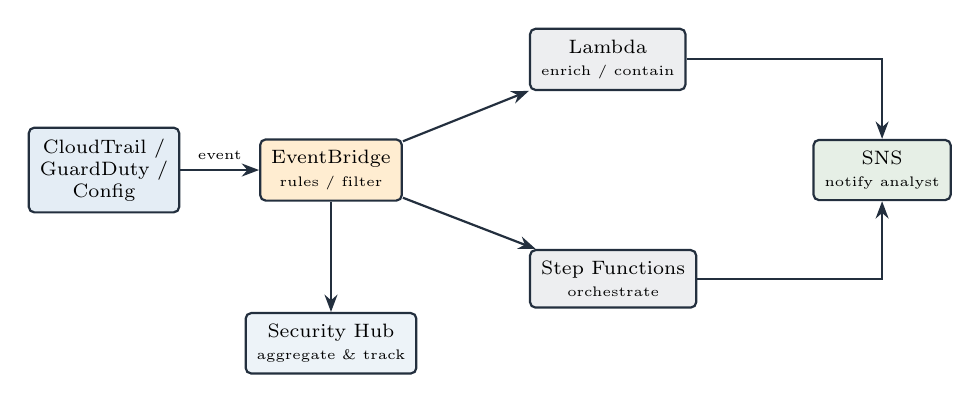
\begin{tikzpicture}[every node/.style={font=\scriptsize},node distance=8mm]
    \node[awsbox,fill=accent!12] (ct) {CloudTrail /\\GuardDuty /\\Config};
    \node[awsbox,right=10mm of ct,fill=awsorange!18] (eb) {EventBridge\\\tiny rules / filter};
    \node[awsbox,above right=6mm and 16mm of eb] (lam) {Lambda\\\tiny enrich / contain};
    \node[awsbox,below right=6mm and 16mm of eb] (sf) {Step Functions\\\tiny orchestrate};
    \node[awsbox,right=52mm of eb,fill=good!12] (sns) {SNS\\\tiny notify analyst};
    \node[awsbox,below=14mm of eb,fill=accent!8] (hub) {Security Hub\\\tiny aggregate \& track};
    \draw[flow] (ct) -- node[above,font=\tiny]{event} (eb);
    \draw[flow] (eb) -- (lam); \draw[flow] (eb) -- (sf);
    \draw[flow] (lam) -| (sns); \draw[flow] (sf) -| (sns);
    \draw[flow] (eb) -- (hub);
  \end{tikzpicture}
  \vspace{0.4em}
  \begin{itemize}\footnotesize
    \item \term{Signal} (CloudTrail/GuardDuty/Config) $\to$ \term{route} (EventBridge) $\to$
          \term{act} (Lambda/Step Functions) $\to$ \term{notify} (SNS) $\to$ \term{track} (Security Hub).
    \item Detection-as-code: rules are version-controlled, tested, and tuned --- not click-ops.
  \end{itemize}
\end{frame}

\begin{frame}{Detection services \& fighting alert fatigue}
  \begin{columns}[T]
    \begin{column}{0.52\textwidth}\footnotesize
      \begin{itemize}
        \item \svc{GuardDuty} --- ML/threat-intel detection (recon, crypto-mining, creds exfil).
        \item \svc{Security Hub} --- normalise \& aggregate findings + posture scoring.
        \item \svc{Config} --- config drift \& compliance rules.
        \item \svc{Inspector} --- vulnerability findings (EC2, ECR images, Lambda).
        \item \svc{Macie} --- sensitive-data exposure in S3.
      \end{itemize}
    \end{column}
    \begin{column}{0.48\textwidth}
      \begin{alertblock}{\footnotesize Alert fatigue is a security risk}
        \footnotesize Too many low-value alerts $\Rightarrow$ real ones are missed.
      \end{alertblock}
      \textbf{\footnotesize Prioritise by:}
      \begin{itemize}\footnotesize
        \item \term{Severity} $\times$ \term{asset criticality} $\times$ \term{exploitability}.
        \item \term{Deduplicate} \& correlate (Security Hub).
        \item \term{Auto-handle} the known-benign; auto-contain the unambiguous.
        \item Track \term{MTTD / MTTR}; tune noisy rules.
      \end{itemize}
    \end{column}
  \end{columns}
\end{frame}

\begin{frame}{Playbooks (1--2): public S3 bucket \& suspicious IAM activity}
  \footnotesize
  \begin{columns}[T]
    \begin{column}{0.5\textwidth}
      \textbf{\color{accent}1. Public S3 bucket detected}\\
      {\tiny Trigger: Config rule / Macie / GuardDuty}
      \begin{itemize}\setlength\itemsep{0pt}
        \item \term{Contain}: Lambda re-applies Block Public Access; remove public statement.
        \item \term{Eradicate}: find root cause (IaC? manual?); fix template; scan for siblings.
        \item \term{Recover}: verify access logs for exfiltration window; rotate exposed data/keys.
        \item \term{Lessons}: add Config guardrail + SCP; alert on \texttt{PutBucketAcl}.
      \end{itemize}
    \end{column}
    \begin{column}{0.5\textwidth}
      \textbf{\color{accent}2. Suspicious IAM activity}\\
      {\tiny Trigger: GuardDuty (anomalous API / new region / creds use)}
      \begin{itemize}\setlength\itemsep{0pt}
        \item \term{Contain}: attach deny-all boundary / disable keys; revoke active sessions.
        \item \term{Eradicate}: identify entry (leaked key? phishing?); remove backdoor users/policies.
        \item \term{Recover}: rotate credentials; restore least-privilege; review CloudTrail timeline.
        \item \term{Lessons}: enforce MFA, kill long-lived keys, add Access Analyzer review.
      \end{itemize}
    \end{column}
  \end{columns}
  \vfill
  {\tiny\color{midgray}Each step is automatable: EventBridge rule $\to$ Lambda/Step Functions $\to$ SNS to the on-call analyst.}
\end{frame}

\begin{frame}{Playbooks (3--4): compromised EC2 \& exposed secret}
  \footnotesize
  \begin{columns}[T]
    \begin{column}{0.5\textwidth}
      \textbf{\color{accent}3. Compromised EC2 instance}\\
      {\tiny Trigger: GuardDuty (C2 / mining / port scan)}
      \begin{itemize}\setlength\itemsep{0pt}
        \item \term{Contain}: swap to isolation SG (no egress); deny instance-role; snapshot for forensics.
        \item \term{Eradicate}: terminate; rebuild from clean AMI via CloudFormation (immutable).
        \item \term{Recover}: redeploy in clean subnet; verify; restore from backup if needed.
        \item \term{Lessons}: patch baseline image; add Inspector scan; review SG exposure.
      \end{itemize}
    \end{column}
    \begin{column}{0.5\textwidth}
      \textbf{\color{accent}4. Exposed secret in a repository}\\
      {\tiny Trigger: secret scanner / push protection}
      \begin{itemize}\setlength\itemsep{0pt}
        \item \term{Contain}: revoke/rotate the secret \emph{immediately} (assume compromised).
        \item \term{Eradicate}: purge from history; remove from artifacts/logs; find reuse.
        \item \term{Recover}: issue new secret via Secrets Manager; audit CloudTrail for misuse.
        \item \term{Lessons}: pre-commit + CI secret scanning; OIDC instead of static keys (Sec.~C/E).
      \end{itemize}
    \end{column}
  \end{columns}
  \vfill
  \bridge{Every playbook reuses Part-I services (CloudTrail, Config, GuardDuty, KMS, Secrets Manager,
  CloudFormation) --- response is \emph{composition}, not new tooling.}
\end{frame}

%##############################################################################
%  PART III -- PRACTICE
%##############################################################################

\begin{frame}[plain,noframenumbering]
  \vfill\centering
  {\color{awsorange}\rule{0.25\paperwidth}{2.5pt}}\\[0.8em]
  {\usebeamerfont{title}\color{awsink}Part III}\\[0.4em]
  {\Large\color{awsink}Exercises, Self-Test \& References}
  \vfill
\end{frame}

%==============================================================================
\section{Exercises \& Self-Test}
%==============================================================================

% \begin{frame}{Additional exercises}
%   \small
%   \begin{enumerate}\setlength\itemsep{4pt}
%     \item \textbf{Zero Trust mapping.} Take the three-tier app (Sec.~D). For each Zero Trust pillar,
%           name one concrete AWS control that enforces it, and one signal that verifies it.
%     \item \textbf{Least privilege.} Given an IAM role with \texttt{"Action":"*"}, rewrite it for a
%           service that only reads from one S3 prefix and writes to one DynamoDB table. Add an MFA condition.
%     \item \textbf{Kubernetes hardening.} List five pod-spec settings that reduce container-escape risk;
%           explain which K8s mechanism enforces each.
%     \item \textbf{Supply chain.} Design a deploy gate that refuses any container image that is unsigned
%           \emph{or} has a critical CVE. Which AWS/CNCF components implement it?
%     \item \textbf{Detection.} Write the EventBridge $\to$ Lambda flow that auto-contains a newly
%           public S3 bucket. What must the Lambda role be allowed to do (least privilege)?
%   \end{enumerate}
% \end{frame}

\begin{frame}{Self-test --- multiple choice (1--4)}
  \footnotesize
  \textbf{Q1.} Under the shared responsibility model for \svc{EKS}, who is responsible for the
  Kubernetes \emph{API server} and \emph{etcd}?\\
  \quad A) Customer \quad B) AWS \quad C) Shared equally \quad D) The CNI plugin vendor

  \vspace{0.6em}
  \textbf{Q2.} The single most important principle of Zero Trust is:\\
  \quad A) Encrypt all disks \quad B) Never trust, always verify \quad
  C) Use a bigger firewall \quad D) Put everything in a private subnet

  \vspace{0.6em}
  \textbf{Q3.} In IAM policy evaluation, which statement is always decisive?\\
  \quad A) An explicit \texttt{Allow} \quad B) The most recent policy \quad
  C) An explicit \texttt{Deny} \quad D) The resource-based policy

  \vspace{0.6em}
  \textbf{Q4.} \term{Dependency confusion} is an attack in which:\\
  \quad A) Two libraries share a function name \quad
  B) An internal package name is resolved to a malicious public package\\
  \quad C) A container cannot find its base image \quad
  D) Two pods get the same service account
\end{frame}

\begin{frame}[fragile]{Self-test --- multiple choice (5--8)}
  \footnotesize
  \textbf{Q5.} Which control best prevents \emph{static AWS credentials} inside EKS pods?\\
  \quad A) Network policies \quad B) IRSA / Pod Identity \quad
  C) A bigger security group \quad D) Read-only root filesystem

  \vspace{0.6em}
  \textbf{Q6.} A \term{permissions boundary} is used to:\\
  \quad A) Grant new permissions \quad B) Cap the maximum permissions an identity can have\\
  \quad C) Encrypt IAM policies \quad D) Replace SCPs

  \vspace{0.6em}
  \textbf{Q7.} Which AWS service answers ``\emph{who} did \emph{what}, \emph{when}, from \emph{where}''?\\
  \quad A) CloudWatch \quad B) Config \quad C) CloudTrail \quad D) Trusted Advisor

  \vspace{0.6em}
  \textbf{Q8.} \term{SLSA} primarily provides:\\
  \quad A) A container runtime \quad B) Build provenance / supply-chain integrity levels\\
  \quad C) A network firewall \quad D) A secrets vault
\end{frame}

\begin{frame}{Self-test --- multiple choice (9--12)}
  \footnotesize
  \textbf{Q9.} In STRIDE, a \emph{public S3 bucket} exposing PII is primarily an instance of:\\
  \quad A) Spoofing \quad B) Tampering \quad C) Information disclosure \quad D) Repudiation

  \vspace{0.6em}
  \textbf{Q10.} The first containment action for an \emph{exposed secret in a repo} is:\\
  \quad A) Open an incident ticket \quad B) Rotate/revoke the secret immediately\\
  \quad C) Delete the repository \quad D) Email all developers

  \vspace{0.6em}
  \textbf{Q11.} Which Kubernetes mechanism is the closest analogue to an AWS \emph{security group}?\\
  \quad A) RBAC Role \quad B) NetworkPolicy \quad C) Admission controller \quad D) Service account

  \vspace{0.6em}
  \textbf{Q12.} To reduce \term{alert fatigue}, the best first step is:\\
  \quad A) Disable GuardDuty \quad B) Forward all alerts to email \quad
  C) Prioritise by severity $\times$ asset criticality \& deduplicate \quad D) Increase log retention
\end{frame}

\begin{frame}{Self-test --- answer key}
  \small
  \begin{columns}[T]
    \begin{column}{0.5\textwidth}
      \begin{tabular}{ll}
        \toprule \textbf{Q} & \textbf{Answer}\\ \midrule
        Q1 & B --- AWS owns the control plane\\
        Q2 & B --- never trust, always verify\\
        Q3 & C --- explicit Deny always wins\\
        Q4 & B --- internal name $\to$ public pkg\\
        Q5 & B --- IRSA / Pod Identity\\
        Q6 & B --- caps maximum permissions\\
        \bottomrule
      \end{tabular}
    \end{column}
    \begin{column}{0.5\textwidth}
      \begin{tabular}{ll}
        \toprule \textbf{Q} & \textbf{Answer}\\ \midrule
        Q7  & C --- CloudTrail\\
        Q8  & B --- build provenance / integrity\\
        Q9  & C --- information disclosure\\
        Q10 & B --- rotate/revoke immediately\\
        Q11 & B --- NetworkPolicy\\
        Q12 & C --- prioritise \& deduplicate\\
        \bottomrule
      \end{tabular}
    \end{column}
  \end{columns}
  \vfill
  {\footnotesize\color{midgray}Score 10+/12 $\Rightarrow$ ready for the lab; review the linked section otherwise.}
\end{frame}

%==============================================================================
\section{References}
%==============================================================================

\begin{frame}{Key takeaways}
  \small
  \begin{itemize}
    \item The customer owns \term{identity, configuration and data} --- that is where breaches happen.
    \item \term{Zero Trust} is the strategy; IAM, VPC, SG, CloudTrail, Config are the tactics.
    \item \term{Containers/Kubernetes} add image, orchestrator and runtime attack surfaces;
          EKS extends the shared-responsibility line at the control plane.
    \item The \term{software supply chain} is production access: sign, attest (SLSA), gate with policy-as-code.
    \item \term{Threat modeling} (STRIDE) turns architecture into a prioritised control list.
    \item \term{Detection \& response} is event-driven and automated: signal $\to$ route $\to$ act $\to$ notify.
  \end{itemize}
  \vfill
  {\footnotesize\color{midgray}Same AWS services throughout --- composed differently for prevention,
  detection and response.}
\end{frame}

\begin{frame}{References \& further reading}
  \footnotesize
  \begin{itemize}\setlength\itemsep{2pt}
    \item AWS Well-Architected Framework --- \emph{Security Pillar}. AWS, current edition.
    \item NIST SP\,800-207 --- \emph{Zero Trust Architecture}. NIST, 2020.
    \item CIS \emph{Kubernetes Benchmark} \& Kubernetes docs --- \emph{Securing a Cluster / Security Best Practices}.
    \item OWASP \emph{Kubernetes Top 10}. OWASP Foundation.
    \item SLSA --- \emph{Supply-chain Levels for Software Artifacts} Framework (\link{slsa.dev}).
    \item OWASP \emph{Software Component Verification Standard (SCVS)}; CycloneDX / SPDX SBOM;
          OWASP \emph{Dependency-Track}.
    \item MITRE ATT\&CK\textsuperscript{\textregistered} --- \emph{Cloud Matrix} (IaaS, Containers).
    \item Cloud Security Alliance --- \emph{Cloud Controls Matrix (CCM)}.
    \item Sigstore / cosign --- artifact \& container signing; in-toto provenance.
    \item Shostack, A. --- \emph{Threat Modeling: Designing for Security}. Wiley, 2014.
    \item AWS Academy --- \emph{Cloud Security Foundations} (base deck for this module).
  \end{itemize}
\end{frame}

\begin{frame}[plain,noframenumbering]
  \vfill\centering
  {\color{awsorange}\rule{0.16\paperwidth}{2.2pt}}\\[0.8em]
  {\usebeamerfont{title}\color{awsink}Thank you}\\[0.4em]
  {\color{midgray}\small Questions, threat models, and counter-examples welcome.}\\[1.0em]
  {\footnotesize\color{midgray}Prof.\ Dr.-Ing.\ Sebastian Schlesinger {\color{awsorange}\textbullet}
   HWR Berlin {\color{awsorange}\textbullet} MSc Cybersecurity}
  \vfill
\end{frame}

\end{document}
